\documentclass[preprint]{elsarticle}
\usepackage{natbib}
\usepackage{bibentry}
\usepackage{amsmath}
\usepackage{amssymb}
\usepackage{amsthm}
\usepackage{amsfonts}
\usepackage{graphicx}
\usepackage{subfigure}
\usepackage{subcaption}
\usepackage{float}
\usepackage{algorithm}
\usepackage{algorithmic}
% Packages for table
\usepackage{multirow}
\usepackage{longtable}
\usepackage{makecell}
\usepackage{array}
\usepackage{booktabs}
\usepackage{hyperref}
\usepackage{comment}
\usepackage{ulem}
\usepackage{etoolbox}
\usepackage{tikz}
\usepackage{geometry}
\usepackage[mathscr]{eucal}
\usepackage{caption}
\newcommand{\mc}[3]{\multicolumn{#1}{#2}{#3}}

%\geometry{a4paper,left=1cm,right=1cm,top=1cm,bottom=1.5cm}

\usepackage{ulem}
\usepackage{color}
\newcommand{\rd}{\textcolor{red}}
\newcommand{\gr}{\textcolor{Green}}
\newcommand{\og}{\textcolor{Orange}}
\newcommand{\ce}{\textcolor{Cerulean}}
\newcommand{\tb}{\textcolor{blue}}

\newtheorem{thm}{Theorem}
\newtheorem{lem}[thm]{Lemma}
\newtheorem{prop}{Proposition}
\newdefinition{rmk}{Remark}
\newdefinition{defn}{Definition}
\newproof{pf}{Proof}
\newproof{pot}{Proof of Theorem \ref{thm2}}

\DeclareMathOperator*{\argmax}{arg\,max}
\DeclareMathOperator*{\argmin}{arg\,min}

\makeatletter
\def\ps@pprintTitle{%
 \let\@oddhead\@empty
 \let\@evenhead\@empty
 \def\@oddfoot{\centerline{\thepage}}%
 \let\@evenfoot\@oddfoot}
\makeatother

\hypersetup{
colorlinks=true,
allcolors=.
}

\title{\textbf{\large{CSE 847 (Spring 2022): Machine Learning --- Project Report}}}
\author[1]{Wei-Chien Liao (\href{mailto:liaowei2@msu.edu}{liaowei2@msu.edu})}
\author[1]{Shihab Shahriar Khan (\href{mailto:khanmd@msu.edu}{khanmd@msu.edu})}
\address[1]{Computer Science and Engineering, Michigan State University}
\date{}

\begin{document}
%\maketitle
\begin{frontmatter}
\begin{abstract}
    This paper is a summary of basic concepts of tensors, Tucker decomposition and higher order singular value decomposition (HOSVD), and variants
    of randomized algorithms for computing these decompositions.
\end{abstract}
\begin{keyword}
    higher order singular value decomposition (HOSVD)\sep Tucker decomposition\sep randomized HOSVD
\end{keyword}
\end{frontmatter}
\section{Introduction}
As we collect ever-increasing amount of data, the importance of creating sophisticated algorithms to analyze and extract meaningful insights out of them is also growing at same pace. A significant subset of this data is multidimensional in nature. They appear naturally in many fields: deep learning [x], Face Recognition [x], solving multi-dimensional integral equations [x] etc. A common characteristics of these data is that they're huge in size- making it hard to apply many traditional machine learning and data analytics tool on this data directly.

\noident One common technique deal to with this is dimension reduction: where these large multi-dimensional arrays (tensors) are transformed into smaller size while maintaining the hidden structures of the data. But straightforward application of even dimension reduction can be prohibitively expensive. A solution to this problem is randomized algorithms. They operate on subsets of data, and has been shown to be quite effective in several application areas [x,x,x].

\noident In this paper, we looked into several randomized algorithms for tensor decomposition. They are:

\begin{itemize}
    \item Random Projection HOSVD (RP-HOSVD)
    \item Random Projection HOOI (RP-HOOI)
    \item Randomized Sequentially Truncated HOSVD (R-STHOSVD)
    \item Randomized Pass-Efficient Algorithm for Tucker Decomposition (R-PET)
\end{itemize}


We implemented these algorithms in Matlab \footnote{https://github.com/williamliao28/CSE847-Project-rHOSVD}, and evaluated their performance, both in terms of reconstruction error and computation time using a real and a synthetic dataset. We show how these randomized variants can significantly reduce computation time while maintaining good reconstruction performance. We also qualitatively evaluated these using image data.


\section{Notation and Preliminaries}
\noindent The contents in this section are mainly based on \cite{Kolda2009}.
\begin{defn}
    The \textbf{order} of a tensor is the number of dimensions, also called \textbf{ways} or \textbf{modes}.
\end{defn}
In this paper,
\begin{itemize}
    \item \textbf{vectors} (tensors of order $1$) are denoeted by boldface lowercase letters, e.g. $\mathbf{a}$.
    \item \textbf{matrices} (tensors of order $2$) are denoeted by boldface capital letters, e.g. $\mathbf{A}$.
    \item \textbf{tensors} (order $\geq 3$) are denoeted by boldface Euler script letters, e.g. $\boldsymbol{\mathscr{X}}$.
    \item the $i$-th entry of a vector $\mathbf{a}$ is denoeted by $a_i$.
    \item the $(i,j)$-th element of a matrix $\mathbf{A}$ is denoeted by $A_{ij}$.
    \item the $(i,j,k)$-th element of a third-order tensor $\boldsymbol{\mathscr{X}}$ is denoeted by $x_{ijk}$.
    \item a colon ``$:$" is used to indicate all elements of a mode. e.g. for a matrix $\mathbf{A}$,
    \begin{itemize}
        \item $\mathbf{a}_{i:} = i$-th row of $\mathbf{A}$.
        \item $\mathbf{a}_{:j} = j$-th column of $\mathbf{A}$.
    \end{itemize}
\end{itemize}
\begin{defn}
    A \textbf{fiber} is defined by fixing every index but one.
\end{defn}
For a third-order tensor $\boldsymbol{\mathscr{X}}$,
\begin{itemize}
    \item $\mathbf{x}_{:jk}=$ \textbf{column fibers} or \textbf{mode-1 fibers}  of $\boldsymbol{\mathscr{X}}$.
    \item $\mathbf{x}_{i:k}=$ \textbf{row fibers} or \textbf{mode-2 fibers}  of $\boldsymbol{\mathscr{X}}$.
    \item $\mathbf{x}_{ij:}=$ \textbf{tube fibers} or \textbf{mode-3 fibers}  of $\boldsymbol{\mathscr{X}}$.
\end{itemize}
\begin{defn}
    \textbf{Slices} are two-dimensional sections of a tensor defined by fixing all but two indices.
\end{defn}
For a third-order tensor $\boldsymbol{\mathscr{X}}$,
\begin{itemize}
    \item $\mathbf{X}_{i::}=$ \textbf{horizontal slices} of $\boldsymbol{\mathscr{X}}$.
    \item $\mathbf{X}_{:j:}=$ \textbf{lateral slices} of $\boldsymbol{\mathscr{X}}$.
    \item $\mathbf{X}_{::k}=$ \textbf{frontal slices} of $\boldsymbol{\mathscr{X}}$.
\end{itemize}
\begin{defn}[Norm of a Tensor]
    The \textbf{norm} of a tensor $\boldsymbol{\mathscr{X}}\in\mathbb{R}^{I_1\times I_2\times\cdots\times I_N}$,
    denoeted by $||\boldsymbol{\mathscr{X}}||$, is defined as
    \begin{equation}
        ||\boldsymbol{\mathscr{X}}||=\sqrt{\sum_{i_1=1}^{I_1}\sum_{i_2=1}^{I_2}\cdots\sum_{i_N=1}^{I_N}x_{i_1i_2\cdots i_N}^2}.
    \end{equation}
\end{defn}
\begin{defn}[Inner Product of Tensors]
    The \textbf{inner product} of two same-sized tensors\\
    $\boldsymbol{\mathscr{X}},\boldsymbol{\mathscr{Y}}\in\mathbb{R}^{I_1\times I_2\times\cdots\times I_N}$,
    denoeted by $\langle\boldsymbol{\mathscr{X}},\boldsymbol{\mathscr{Y}}\rangle$, is defined as
    \begin{equation}
        \langle\boldsymbol{\mathscr{X}},\boldsymbol{\mathscr{Y}}\rangle=\sqrt{\sum_{i_1=1}^{I_1}\sum_{i_2=1}^{I_2}\cdots\sum_{i_N=1}^{I_N}x_{i_1i_2\cdots i_N}y_{i_1i_2\cdots i_N}}.
    \end{equation}
\end{defn}
Thus, by the definition of norm and inner product,
$\langle\boldsymbol{\mathscr{X}},\boldsymbol{\mathscr{X}}\rangle=||\boldsymbol{\mathscr{X}}||^2$.
\begin{defn}[Rank-one Tensors]
    A $N$-way tensor $\boldsymbol{\mathscr{X}}\in\mathbb{R}^{I_1\times I_2\times\cdots\times I_N}$ is \textbf{rank one} if it can
    be written as the outer product of $N$ vectors,
    \begin{equation}
        \boldsymbol{\mathscr{X}} = \mathbf{a}^{(1)}\circ\mathbf{a}^{(2)}\circ\cdots\circ\mathbf{a}^{(N)},
    \end{equation}
    for some vectors $\mathbf{a}^{(1)},\mathbf{a}^{(2)},\cdots,\mathbf{a}^{(N)}$ and ``$\circ$'' denotes the vector outer product.
\end{defn}
\begin{defn}
    A tensor is called \textbf{cubical} if every mode is the same size. A cubical tensor is called \textbf{supersymmetric}
    (some literatures call this ``symmetric'') if its elements remain constant under any permutation of the indices.
\end{defn}
For a $3$-way tensor $\boldsymbol{\mathscr{X}}\in\mathbb{R}^{I\times I\times I}$, it is supersymmetric if
\[
    x_{ijk} = x_{ikj} = x_{jik} = x_{jki} = x_{kij} = x_{kji} \quad \forall i,j,k=1,\cdots I.
\]
\begin{defn}[Diagnoal Tensor]
    A tensor $\boldsymbol{\mathscr{X}}\in\mathbb{R}^{I_1\times I_2\times\cdots\times I_N}$ is \textbf{diagonal}
    if $x_{i_1i_2\cdots i_N}\neq 0$ only if $i_1=i_2=\cdots=i_N$. 
\end{defn}
\begin{defn}[Matricization]
    The process of reordering the elements of an $N$-way array into a matrix is called \textbf{matricization}
This is also called \textbf{unfolding} or \textbf{flattening}.
\end{defn}
The mode-$n$ matricization of a tensor $\boldsymbol{\mathscr{X}}\in\mathbb{R}^{I_1\times I_2\times\cdots\times I_N}$
is denoeted by $\mathbf{X}_{(n)}$ and arranges the mode-$n$ fibers to be the columns of the resulting matrix.
\begin{rmk}
    It is also possible to vectorize a tensor. This process is called vectorization.
\end{rmk}
\subsection{Tensor Mulitiplication}
\noindent The \textbf{$n$-mode prodcut} of a tensor $\boldsymbol{\mathscr{X}}\in\mathbb{R}^{I_1\times I_2\times\cdots\times I_N}$
with a matrix $\mathbf{U}\in\mathbb{R}^{J\times I_n}$ is defined as
\begin{subequations}
    \begin{align}
        & \text{eletmenwise: } \quad \left(\boldsymbol{\mathscr{X}}\times_n\mathbf{U}\right)_{i_1\cdots i_{n-1}ji_{n+1}\cdots i_N}
        =\sum_{i_n=1}^{I_n}x_{i_1i_2\cdots i_N}u_{ji_n} \\
        & \text{unfold tensors: } \quad \boldsymbol{\mathscr{Y}} = \boldsymbol{\mathscr{X}}\times_n\mathbf{U}\Leftrightarrow
        \mathbf{Y}_{(n)} = \mathbf{U}\mathbf{X}_{(n)}
    \end{align}
\end{subequations}
The result is a tensor of size $I_1\times\cdots\times I_{n-1}\times J\times I_{n+1}\times\cdots\times I_N$. Each mode-$n$ fiber is multiplied by the matrix $\mathbf{U}$.
The following are some properties of the $n$-mode prodcut:
\begin{enumerate}
    \item[(1)] For distinct modes
    in a series of multiplications, the order of the multiplication is irrelevant.
    \begin{equation}
        \boldsymbol{\mathscr{X}}\times_m\mathbf{A}\times_n\mathbf{B} = \boldsymbol{\mathscr{X}}\times_n\mathbf{B}\times_m\mathbf{A},\quad \text{for } n\neq m.
    \end{equation}
    \item[(2)] If the modes are the same
    \begin{equation}
        \boldsymbol{\mathscr{X}}\times_n\mathbf{A}\times_n\mathbf{B}=\boldsymbol{\mathscr{X}}\times_n(\mathbf{B}\mathbf{A}).
    \end{equation} 
\end{enumerate}
\subsection{Some Matrix Products}
\begin{itemize}
    \item \underline{\textbf{Kronecker Product}}\\[0.3cm]
    The \textbf{Kronecker product} of two matrices $\mathbf{A}\in\mathbb{R}^{I\times J}$ and $\mathbf{B}\in\mathbb{R}^{K\times L}$,
    denoeted by $\mathbf{A}\otimes\mathbf{B}$, is defined as
    \begin{equation}
        \mathbf{A}\otimes\mathbf{B}=\begin{bmatrix}
            a_{11}\mathbf{B} & a_{12}\mathbf{B} & \cdots & a_{1J}\mathbf{B} \\
            a_{21}\mathbf{B} & a_{22}\mathbf{B} & \cdots & a_{2J}\mathbf{B} \\
            \vdots & \vdots & \ddots & \vdots \\
            a_{I1}\mathbf{B} & a_{I2}\mathbf{B} & \cdots & a_{IJ}\mathbf{B}
        \end{bmatrix}
    \end{equation}
    \item \underline{\textbf{Khatri-Rao Product}}\\[0.3cm]
    The \textbf{Khatri-Rao product} of two matrices $\mathbf{A}\in\mathbb{R}^{I\times K}$ and $\mathbf{B}\in\mathbb{R}^{J\times K}$,
    denoeted by $\mathbf{A}\odot\mathbf{B}$, is defined as
    \begin{equation}
        \mathbf{A}\odot\mathbf{B}=\begin{bmatrix}
            \mathbf{a}_{1}\otimes\mathbf{b}_1 & \mathbf{a}_{2}\otimes\mathbf{b}_2 & \cdots & \mathbf{a}_{K}\otimes\mathbf{b}_K
        \end{bmatrix}
    \end{equation}
    \item \underline{\textbf{Hadamard Product}}\\[0.3cm]
    The \textbf{Hadamard product} of two matrices $\mathbf{A}, \mathbf{B}\in\mathbb{R}^{I\times J}$,
    denoeted by $\mathbf{A}*\mathbf{B}$, is defined as
    \begin{equation}
        \mathbf{A}*\mathbf{B}=\begin{bmatrix}
            a_{11}b_{11} & a_{12}b_{12} & \cdots & a_{1J}b_{1J} \\
            a_{21}b_{21} & a_{22}b_{22} & \cdots & a_{2J}b_{2J} \\
            \vdots & \vdots & \ddots & \vdots \\
            a_{I1}b_{I1} & a_{I2}b_{I2} & \cdots & a_{IJ}b_{IJ}
        \end{bmatrix}
    \end{equation}
\end{itemize}
Some properties of these matrix prodcuts:
\begin{subequations}
    \begin{align}
        (\mathbf{A}\otimes\mathbf{B})(\mathbf{C}\otimes\mathbf{D}) &= \mathbf{A}\mathbf{C}\otimes\mathbf{B}\mathbf{D} \\
        (\mathbf{A}\otimes\mathbf{B})^{\dagger} &= \mathbf{A}^{\dagger}\otimes\mathbf{B}^{\dagger} \\
        \mathbf{A}\odot\mathbf{B}\odot\mathbf{C} &= (\mathbf{A}\odot\mathbf{B})\odot\mathbf{C} = \mathbf{A}\odot(\mathbf{B}\otimes\mathbf{C}) \\
        (\mathbf{A}\odot\mathbf{B})^T(\mathbf{A}\odot\mathbf{B}) &= (\mathbf{A}^T\mathbf{A})*(\mathbf{B}^T\mathbf{B}) \\
        (\mathbf{A}\odot\mathbf{B})^{\dagger} &= (\mathbf{A}^T\mathbf{A})*(\mathbf{B}^T\mathbf{B})^{\dagger}(\mathbf{A}\odot\mathbf{B})^T
    \end{align}
\end{subequations}
\section{Higher Order Singular Value Decomposition (HOSVD)}
\noindent This section aims to explain the basic concepts of HOSVD. The HOSVD can be viewed as a form of higher-order
principal component analysis (PCA). Different names of HOSVD appear in literatures including Tucker Decomposition, 
$N$-mode PCA, or $N$-mode SVD. The core concept of HOSVD is to decomposes a tensor into a core tensor multiplied
(or transformed) by a matrix along each mode. To express this idea in mathematical equation, we first consider the
three-way case, then extend it to general $N$-way tensors.
\vskip 0.3cm
\noindent Let $\boldsymbol{\mathscr{X}}\in\mathbb{R}^{I\times J\times K}$ be a three-way tensor. The HOSVD of $\boldsymbol{\mathscr{X}}$
is defined as
\begin{equation}
    \boldsymbol{\mathscr{X}}\approx \boldsymbol{\mathscr{G}}\times_1\mathbf{A}\times_2\mathbf{B}\times_3\mathbf{C}
    = \sum_{p=1}^P\sum_{q=1}^Q\sum_{r=1}^R g_{pqr}\mathbf{a}_p\circ\mathbf{b}_q\circ\mathbf{c}_r
    = [\![\boldsymbol{\mathscr{G}}\ ; \ \mathbf{A}, \ \mathbf{B}, \ \mathbf{C}]\!].
\end{equation}
where $\mathbf{A}\in\mathbb{R}^{I\times P}$, $\mathbf{B}\in\mathbb{R}^{J\times Q}$, and $\mathbf{C}\in\mathbb{R}^{K\times R}$ are called the \textbf{factor matrices},
and $\boldsymbol{\mathscr{G}}\in\mathbb{R}^{P\times Q\times R}$ is called the \textbf{core tensor}. The factor matrices
can be thought of as the principal components in each mode similar to the case in SVD, and entries of the core tensor show
he level of interaction between the different components. Thus, this is similar to the 
singular value matrix in SVD in some sense. This can also be written in eletmenwise form as follows
\begin{equation}
    x_{ijk}\approx\sum_{p=1}^P\sum_{q=1}^Q\sum_{r=1}^R g_{pqr}a_{ip}b_{jq}c_{kr} \quad \text{for } i=1,\cdots,I, \ j=1,\cdots,J, \
    k=1,\cdots, K.
\end{equation}
Note that the factor matrices are not assumed to be orthogonal or columnwise orthonormal, but it is possible make factor matrices
to have these desired properties. HOSVD can also be written in matricized form,
\begin{equation}
    \begin{aligned}
        & \mathbf{X}_{(1)}\approx \mathbf{A}\mathbf{G}_{(1)}\left(\mathbf{C}\otimes\mathbf{B}\right)^T \\
        & \mathbf{X}_{(2)}\approx \mathbf{B}\mathbf{G}_{(2)}\left(\mathbf{C}\otimes\mathbf{A}\right)^T \\
        & \mathbf{X}_{(3)}\approx \mathbf{C}\mathbf{G}_{(3)}\left(\mathbf{B}\otimes\mathbf{A}\right)^T
    \end{aligned}
\end{equation}
\vskip 0.3cm
\noindent For a general $N$-way tensor $\boldsymbol{\mathscr{X}}\in\mathbb{R}^{I_1\times I_2\times\cdots\times I_N}$, the
HOSVD can be generalized as
\begin{equation}
    \boldsymbol{\mathscr{X}}\approx \boldsymbol{\mathscr{G}}\times_1\mathbf{A}^{(1)}\times_2\mathbf{A}^{(2)}\cdots\times_N\mathbf{A}^{(N)}
    = [\![\boldsymbol{\mathscr{G}}\ ; \ \mathbf{A}^{(1)}, \ \mathbf{A}^{(2)}, \cdots, \mathbf{A}^{(N)}]\!].
\end{equation}
Expressing this elementwise gives
\begin{equation}
    x_{i_1i_2\cdots i_N}\approx\sum_{r_1=1}^{R_1}\sum_{r_2=1}^{R_2}\cdots\sum_{r_N=1}^{R^N} g_{r_1r_2\cdots r_N}a_{i_1r_1}^{(1)} a_{i_2r_2}^{(2)}\cdots 
    a_{i_Nr_N}^{(N)} \quad \text{for } i_n=1,\cdots,I_n, \ n=1,\cdots,N.
\end{equation}
The matricized version is given by
\begin{equation}
    \mathbf{X}_{(n)}\approx \mathbf{A}^{(n)}\mathbf{G}_{(n)}\left(\mathbf{A}^{(N)}\otimes\cdots\otimes\mathbf{A}^{(n+1)}
    \otimes\mathbf{A}^{(n-1)}\otimes\cdots\otimes\mathbf{A}^{(1)}\right)^T,
\end{equation}
for $n=1,2,\cdots, N$.
\vskip 0.3cm
\noindent The following definition of $n$-rank, sometimes called numerical rank or multilinear rank in some literatures, is useful for study algorithms
corresponding to HOSVD.
\begin{defn}[n-rank]
    $\boldsymbol{\mathscr{X}}\in\mathbb{R}^{I_1\times I_2\times\cdots\times I_N}$ be a $N$-way tensor. Then the \textbf{n-rank}
    of $\boldsymbol{\mathscr{X}}$, denoted by $\text{rank}_n(\boldsymbol{\mathscr{X}})$, is the column rank of $\mathbf{X}_{(n)}$.
\end{defn}
Thus, the n-rank of a tensor is the dimension of the vector space spanned by the mode-$n$ fibers. With this terminology,
if let $R_n = \text{rank}_n(\boldsymbol{\mathscr{X}})$, then the tensor $\boldsymbol{\mathscr{X}}$ can be called a
rank-$(R_1,R_2,\cdots,R_N)$ tensor.
\subsection*{Algorithms for Computing HOSVD}
\noindent Common algorithms for computing the HOSVD of a given tensor $\boldsymbol{\mathscr{X}}$ include ``classical" HOSVD, Sequentially Truncated HOSVD (STHOSVD), and
Higher-Order Orthogonal Iteration (HOOI).
\vskip 0.3cm
\noindent The ``classical" HOSVD simply perform SVD to compute the left singular vectors of $\mathbf{X}_{(n)}$ for each $n$,
then form the core tensor. Although this is straightforward, it is inefficient for large tensor data since performing SVD
is computationally expensive.
\vskip 0.3cm
\noindent The Sequentially Truncated HOSVD (STHOSVD) reduce the comoputation complexity by sequentially shrink the size of
the underlying unfolding matrices used as input for SVD in each iteration. The SVD decompositions for $\mathbf{X}_{(n)}$ in ``classical'' HOSVD
is now replaced by truncated SVD. This not only greatly enhance the speed without sacrficing the accuracy, and sometimes even
gives better accuracy. However, this method does not guarantee to find the best multilinear rank approximation for a given tensor.
\vskip 0.3cm
\noindent An alternative way to deal with the high computational complexity of ``classical'' HOSVD is to observe that the problem
of finding the left singular vectors of can be reformulated as solving equivalent least squares problems. This type of methods has the advantage that
the result output would provide numerically the best multilinear rank approximation for a tensor.
The Higher-Order Orthogonal Iteration (HOOI) algorithm is developed based on this observation. If the HOSVD of the tensor
$\boldsymbol{\mathscr{X}}\in\mathbb{R}^{I_1\times I_2\times\cdots\times I_N}$ is given by
\[
    \boldsymbol{\mathscr{X}}\approx \boldsymbol{\mathscr{G}}\times_1\mathbf{Q}^{(1)}\times_2\mathbf{Q}^{(2)}\cdots\times_N\mathbf{Q}^{(N)}  
\]
Write this in matricized form to obtain for each $n=1,2,\cdots,N$,
\[
    \mathbf{X}_{(n)}\approx \mathbf{Q}^{(n)}\mathbf{G}_{(n)}\left(\mathbf{Q}^{(N)}\otimes\cdots\otimes\mathbf{Q}^{(n+1)}
    \otimes\mathbf{Q}^{(n-1)}\otimes\cdots\otimes\mathbf{Q}^{(1)}\right)^T.
\]
Assume the factor matrix $\mathbf{Q}^{(n)}$ is unknown and other factor matrices are known, then $\mathbf{Q}^{(n)}$
can be computed by solving the following least square problem,
\begin{equation}
    \mathbf{Q}^{(n)} = \argmin_{\mathbf{Q}\in\mathbb{R}^{I_n\times R_n}}||\mathbf{A}^{(n)}\mathbf{Q}^T-\mathbf{X}_{(n)}^T||_F^2,
\end{equation}
where
\[
    \mathbf{A}^{(n)} = \left(\mathbf{Q}^{(N)}\otimes\cdots\otimes\mathbf{Q}^{(n+1)}
    \otimes\mathbf{Q}^{(n-1)}\otimes\cdots\otimes\mathbf{Q}^{(1)}\right)\mathbf{G}_{(n)}^T.
\]
This is equivalent to finding the left singular vectors of the matrix $\mathbf{Z}_{(n)}$, where
the corresponding tensor $\boldsymbol{\mathscr{Z}}$ is defined by
\[
    \boldsymbol{\mathscr{Z}} := \boldsymbol{\mathscr{X}}\times_{k\neq n}\left\{\mathbf{Q}^{(n)}\right\}^T.
\]
Repeat this process for each $n=1,\cdots, N$. Then compute the core tensor $\boldsymbol{\mathscr{G}}$
by solving the following equivalent least square problem
\begin{equation}
    \boldsymbol{\mathscr{G}}=\argmin_{\boldsymbol{\mathscr{G}}\in\mathbb{R}^{R_1\times R_2\times\cdots\times R_n}}
    ||\mathbf{B}\mathbf{g}-\mathbf{x}||_2^2,
\end{equation}
where $\mathbf{g}$ and $\mathbf{x}$ are vectorization of the tensors $\boldsymbol{\mathscr{G}}$ and
$\boldsymbol{\mathscr{X}}$ respectively.
\begin{rmk}
Unlike the SVD of a matrix, the HOSVD of a tensor is not guaranteed to be unique. A more detailed discussion
can be found in section 4.3 of \cite{Kolda2009}.
\end{rmk}
\section{Randomized Algorithms for Computing HOSVD}
\noindent This section summarizes some randomized algorithm for computing HOSVD discussed in \cite{9350569}. The HOSVD algorithms
described in the previous section has a common challenge that it is expensive to compute low-rank approximation of the unfolding matrices.
In view of this issue, many algorithms are developed based on introducing randomized low-rank matrix algorithms to replace the truncated SVD or
economic SVD used in HOSVD algorithms.
These randomized algorithms can be mainly classifed as the following four types: random projecttion,
randomized sampling, randomized count-sketch, and randomized least-squares. There are also new algorithms, such as the Sketched
alternating least-squares (ALS) proposed in \cite{ma2021fast}, which combines count-sketch and random least-squares techniques.
\subsection{Random Projection}
\noindent The basic idea of random projection class algorithms is to approximate the column space of the unfolding matrices of a given data tensor
as follows: let $\mathbf{X}\in\mathbb{R}^{m\times n}$ denote the original data matrix.
\begin{enumerate}
    \item Generate a random matrix $\mathbf{\Omega}\in\mathbb{R}^{n\times p}$ with $p<n$ from some probability distribution such as 
    Gaussian, Bernoulli or uniform distribution.
    \item Compute $\mathbf{Y}=\mathbf{X}\mathbf{\Omega}\in\mathbb{R}^{m\times p}$.
\end{enumerate}
Then this new matrix $\mathbf{Y}$ has $p$ column vectors randomly generated from the column space of $\mathbf{X}$ and has 
fewer columns than the original $\mathbf{X}$.
\vskip 0.3cm
\noindent Based on this concept, the ``classical'' HOSVD, STHOSVD, and HOOI can be modified by adding this techniques and gives
the Random Projection HOSVD (RP-HOSVD) algorithm, the Randomized STHOSVD (R-STHOSVD) algorithm and the Random Projection HOOI (RP-HOOI)
algorithm respectively. An issue of the above three randomized algorithms is that they all require passing the input data tensor multiple times.
This could produce high communication costs if the data tensors are stored on multiple cores. Hence, a class of algorithms refeered to as
Randomized Pass-Efficient algorithms (such as R-PET) are proposed to remedy this issue.
\subsection{Randomized Sampling}
\noindent The main idea of this class of methods is to compute the factor matrices by sampling the columns or rows
of the corresponding unfolding matrix of the input data tensor. There are many different sampling techniques that can
be applied to randomly select the columns or rows. The sampling can be based on probability distributions like
Gaussian distribution or uniform distribution. It is also possible to consider sampling with or without replacement.
There are other techniques like sampling based on leverage score and cross-approximation that can also be applied to the
sampling step of this class of algorithms. Some examples of algorithms belonging to this class are
Randomized Sampling Tucker Approximation (R-ST) and Randomized Higher Order Interpolatory Decomposition (R-HOID).
\subsection{Randomized Least-squares}
\noindent The motivation of developing this type of algorithms is that RP-HOOI requires several multiplications of random matrices and operations of the core tensors
with factor matrices. This becomes expensive if it needs many iterations to converge. This class of methods aims to reduce this cost by
replacing these costly computations by some equivalent least squares problems. As shown in the previous section, computing the HOSVD of a tensor
can be transformed to an equivalent optimization problem which can then be reformulated as solving some least squares problems.
\subsection{Randomized Count-sketch}
\noindent Similar to the idea of random projection, count-sketch also aims to generate random vectors in the column 
or row space spanned by the original data matrix. In random project, it requires to perform matrix multiplication of original data matrix
and a random matrix. This could be expensive when coping with large data. Count-sketch attempts to cure this problem by generating the desired
vectors without comoputing matrix multiplications. The procedure of count-sketch can be summarized into the
following three steps:
\begin{enumerate}
    \item Hashing
    \item Distributing vectors with same hash numbers to the same group
    \item Signing the columns and summing each group as a representative column
\end{enumerate}
This kind of techniques can be applied to tensors with some proper extensions. This technique is applied in RP-HOOI
to solve the underlying least squares problems.

\pagebreak
\section{Numerical Results}

\subsection{Datasets and Experimental Details}
\noindent We used two datasets for experiments. First one is a synthetic dataset of shape $1000\times1000\times1000$ following the procedure outlined in \cite{9350569}. To create the dataset, we first generate a core tensor $S \in   \mathbb{R}^{1000\times1000\times1000}$, and three factor matrices $Q1 \in \mathbb{R}^{1000\times40}$, $Q2 \in \mathbb{R}^{1000\times20}$ and $Q3 \in \mathbb{R}^{1000\times30}$. The data tensor $X$ was then generated by multipying core tensor with three factor matrices.

\noindent The second dataset is a real-world video dataset. The video contains 2400 RGB frames of shape $1080\times1920\times$. We converted the video to grayscale, and took the first 300 frames to generate a tensor $X \in \mathbb{R}^{300\times1080\times1920}$.

\noindent The experiments were carried out in an intel-18 instance from MSU HPCC cluster with 96GB RAM and 32 cores. All tensor decomposition algorithms were implemented in Matlab. Python was used to modify data and plot figures. 

\noindent The reconstruction performance was evaluated using reconstruction error E:

\begin{equation*}
    E = \frac{{\lVert X-\^{X} \rVert}_F}{{\lVert X \rVert}_F}
\end{equation*}

\noindent Where $X$ is given data and $\^{X}$ is the tucker approximation.

\subsection{Quantitative Results}


\begin{figure}[h]
    \centering
    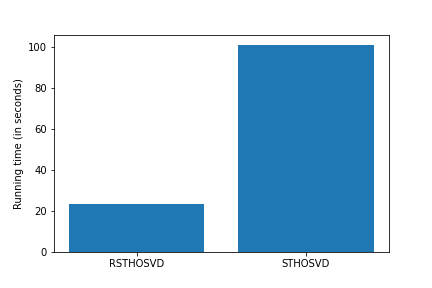
\includegraphics[scale=0.7]{figs/rVSd.png}
    \caption{Randomized vs deterministic tensor decomposition.}
    \label{rvsd}
\end{figure}

We begin by demonstrating the computational efficiency of randomized algorithms over their deterministic counterparts. Figure \ref{rvsd} shows time taken by both algorithms for Video dataset. Both algorithms' parameters were tuned such that reconstruction error $E=1.8e-2$. Deterministic STHOSVD took around 100 seconds to complete, whereas randomized variant RSTHOSVD too little less than 25 seconds, a 4x speedup. Our experiments showed the relative speedup increases as dataset grows, so the performance difference is expected to be even higher for larger tensors. 

We next show the relative performance of several randomized algorithms we implemented using the synthetic dataset. As Figure \ref{fig:booh} shows, the performance is comparable among the algorithms, RPHOSVD has a slight edge over others. 

\begin{figure}
    \centering
    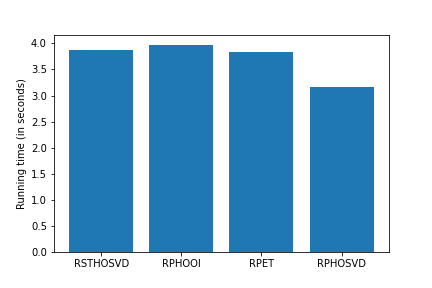
\includegraphics[scale=.7]{figs/runtime.png}
    \caption{Performance of random tensor decomposition algorithms.}
    \label{fig:booh}
\end{figure}

Lastly, the reconstruction and computational performance of all algorithms, including deterministic STHOSVD are presented in table 1.

\begin{center}
\captionof{table}{Relative error and time comparison of different algorithms using synthetic data.}
\begin{tabular}{lll}
\toprule
  Method & Time Taken & Reconstruction Error \\
\midrule
 STHOSVD &       3.27 &             3.42e-15 \\
RSTHOSVD &        3.8 &             1.27e-12 \\
  RPHOOI &       3.97 &             1.18e-14 \\
    RPET &       3.83 &            1.543e-10 \\
 RPHOSVD &       3.16 &             1.00e-13 \\
\bottomrule
\end{tabular}
\end{center}

\subsection{Qualitative Results}
We show the reconstruction performance on 50th frame of our video dataset.

\begin{figure}[h!]
    \centering
    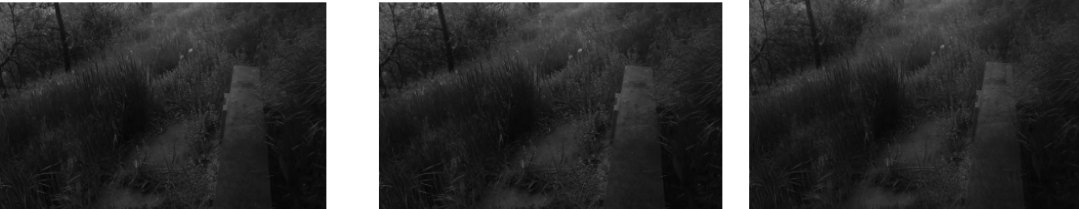
\includegraphics[width=\textwidth]{figs/osr.png}
    \caption{Left: Original image. Middle: reconstructed from STHOSVD, Right: Reconstruction from RSTHOSVD.}
    \label{fig:my_label}
\end{figure}

The one using ra

\subsection{Limitations}

\section{Conclusion}
\bibliographystyle{plain}
\bibliography{msu-cse847-project}
\end{document}